\chapter{Green関数}
\section{Green関数の一般形}
\subsection{数学寄りの定義}
\begin{itembox}[c]{Green関数}
  ある微分演算子${\cal D}$について
  \begin{eqnarray}
    {\cal D}G(x, x') = \delta(x-x')
  \end{eqnarray}
  が成立するとき,$G$を${\cal D}$に対するGreen関数と呼ぶ.
\end{itembox}
ただし, 境界条件がないと$G(x, x')$は一意に決まらない.
\subsection{物理寄りの定義}
ある線形エルミート演算子$L$が
\begin{eqnarray}
  L\ket{a} = \ket{a}
\end{eqnarray}
のように定義されているとする. $\ket{a}$の形式解は
\begin{eqnarray}
  \ket{a} = L^{-1}\ket{a}\label{greenian}
\end{eqnarray}
のように表される. このとき$L^{-1}$をGreen演算子と呼び$L^{-1} = G$と書く. (\ref{greenian})を任意の連続基底\footnote{生成消滅演算子の固有状態などを持ってくると基底は離散になってしまうのでDelta関数が現れない.}で縮約を取り, 完全系を用いて式変形をする:
\begin{eqnarray}
  \expval{l|a} &=& \bra{l}G\ket{a}\\
  &=& \int dl' \bra{l}G\ket{l'}\expval{l'|a}\\
  \Bigl(&=& \int dl' G(l,l')\psi(l', a)\Bigr)
\end{eqnarray}
このとき, $\bra{l}G\ket{l'}$を演算子$L$に対するGreen関数と呼ぶ.

ここで定常Schr\"odinger方程式
\begin{eqnarray}
  (E-\hat{H})\psi(x) = 0 \Longleftrightarrow \hat{L}\psi(x) = 0
\end{eqnarray}
が与えられたとする. $\hat{L}$に対するGreen関数は$G = (E-\hat{H})^{-1}$と表される. また
\begin{eqnarray}
  \hat{L}G = (E-\hat{H})G = I
\end{eqnarray}
という関係に左右からハミルトニアンの固有状態\footnote{固有状態でないと$\bra{x}(E-\hat{H})\ket{x''} = (E-H)\expval{x|x''}$のような変形が正当化されない.}を作用させると
\begin{eqnarray}
  \bra{x}(E-\hat{H})G\ket{x'} &=& \bra{x}I\ket{x'}\\
  \int dx''\bra{x}(E-\hat{H})\ket{x''}\bra{x''}G\ket{x'}&=& \delta(x-x')\\
  \int dx''(E-H)\delta(x - x'')\bra{x''}G\ket{x'}&=& \delta(x-x')
\end{eqnarray}
よって見慣れた形式
\begin{eqnarray}
  (E-H)G(x, x') = \delta(x-x')
\end{eqnarray}
を得る.
\subsection{Green演算子のスペクトル表示}
生成消滅演算子の粒子数状態の完全系を用いて
\begin{eqnarray}
  G = (E-\hat{H})^{-1} &=& \sum_{nn'}\ket{n}\bra{n}(E-\hat{H})^{-1}\ket{n'}\bra{n'}\\
  &=& \sum_{nn'}(E-E_n)^{-1}\ket{n}\bra{n'}\delta_{nn'}\\
  &=& \sum_{nn'}\frac{\ket{n}\bra{n}}{(E-E_n)}
\end{eqnarray}
と表すことができる. ただし, ハミルトニアンが生成消滅演算子の2次形式で記述できていなければならない.
\section{量子力学とGreen関数}
\subsection{摂動展開とGreen関数}
定常シュレディンガー方程式
\begin{eqnarray}
  H\psi(x) = E\psi(x)\label{schroe}
\end{eqnarray}
が与えられており, ハミルトニアンは
\begin{eqnarray}
  H = H_u + H_p
\end{eqnarray}
と書けるものとする. $H_u, H_p$はそれぞれ非摂動ハミルトニアン, 摂動ハミルトニアンである\footnote{摂動部を解析的に解ける線形項に, 非摂動部を解析的に解けない非線形項にするのが一般的. 量子力学において解析的に解けるものは調和振動子くらいしかないが, 生成消滅演算子の2次形式になってさえいればBogoliubov変換などを通して対角化が可能な形式にできる. 一方相互作用項は非線形(生成消滅演算子の4次)になっているので解析的に解けない.}. (\ref{schroe})を変形する:
\begin{eqnarray}
  (E-H_u)\psi(x) = H_p\psi(x)
\end{eqnarray}
非摂動ハミルトニアンを線形演算子として線形演算子$L_u$及びGreen関数$G_u$を定義する:
\begin{eqnarray}
  L_u = E-H_u\hspace{1cm}G_u = (E-H_u)^{-1}
\end{eqnarray}
さらに, Schr\"odinger方程式は
\begin{eqnarray}
  (L_0-H_p)\psi(x) = 0
\end{eqnarray}
と書け, この式のGreen関数は
\begin{eqnarray}
  G = (L_0 - H_p)^{-1}
\end{eqnarray}
である. ここで, 一般に非可換な演算子$A, B$に対する逆演算子は
\begin{eqnarray}
  \frac{1}{A} &=& \frac{1}{B} + \frac{1}{B}(B-A)\frac{1}{A}\\
  &=& \frac{1}{B} + \frac{1}{B}(B-A)\left(\frac{1}{B} + \frac{1}{B}(B-A)\frac{1}{A}\right)\\
  &=& \frac{1}{B} + \frac{1}{B}(B-A)\frac{1}{B} + \frac{1}{B}(B-A)\frac{1}{B}(B-A)\frac{1}{A}\\
  &=& \frac{1}{B} + \frac{1}{B}(B-A)\frac{1}{B} + \frac{1}{B}(B-A)\frac{1}{B}(B-A)\left(\frac{1}{B} + \frac{1}{B}(B-A)\frac{1}{A}\right)\\
  \nonumber    &=& ...
\end{eqnarray}
のように逐次展開を繰り返すことができる. $A \rightarrow A - B,\ B \rightarrow A$と変形することにより
\begin{eqnarray}
  \frac{1}{A-B} = A^{-1} + A^{-1}BA^{-1} + A^{-1}BA^{-1}BA^{-1} + ...
\end{eqnarray}
という公式を得る. これを用いると
\begin{eqnarray}
  G = \frac{1}{L_u - H_p} &=& L_u^{-1} + L_u^{-1}H_pL_u^{-1} + L_u^{-1}H_pL_u^{-1}H_pL_u^{-1} + ...\\
  &=& G_0 + G_0H_pG_0 + G_0H_pG_0H_pG_0 + ...\\
  &=& G_0 + G_0H_pG = G_0 + GH_pG_0
\end{eqnarray}
のように, FullのハミルトニアンのGreen関数は非摂動Green関数を用いて展開できる.

ここで, ハミルトニアン$\hat{H} = \hat{H}_u+\hat{H}_p$の固有状態$\ket{n}$について
\begin{eqnarray}
  (E-\hat{H})\ket{n} &=& 0\\
  (E-\hat{H}_u)\ket{n} &=& \hat{H}_p\ket{n}\\
  \ket{n} = \frac{\hat{H}_p}{E-\hat{H}_u}\ket{n} &=& G_u\hat{H}_p\ket{n}
\end{eqnarray}
が成立している. さらに左から$\bra{x}$を作用させる:
\begin{eqnarray}
  \expval{x|n} &=& \int dx'dx''\bra{x}G_u\ket{x''}\bra{x''}\hat{H}_p\ket{x'}\expval{x'|n}\\
  \psi_n(x) &=& \int dx'dx''G_u(x, x'')H_p(x')\delta(x'-x'')\psi_n(x')\\
  &=& \int dx'G_u(x, x')H_p(x')\psi_n(x')
\end{eqnarray}
$\bra{x}$を作用させるのは$x$表示にして微分方程式を解くようなものなので, これには境界条件が足りない. $H_p = 0$, つまり摂動項がない場合の特解を$\expval{x|n}_0 = \psi_{0n}(x)$とすると
\begin{eqnarray}
  \psi_n(x) &=& \psi_{0n}(x) + \int dx'G_u(x, x')H_p(x')\psi_n(x')
\end{eqnarray}
となる. ただしこれはあくまで形式解である. 両辺に未知関数$\psi_n(x)$があるので, 繰り返し代入することで展開していく:
\begin{eqnarray}
  \nonumber    \psi_n(x) &=& \psi_{0n}(x) + \int dx'G_u(x, x')H_p(x')\left[\psi_{0n}(x') + \int dx''G_u(x', x'')H_p(x'')\psi_n(x'')\right]\\
  \nonumber     &=& \psi_{0n}(x) + \int dx'G_u(x, x')H_p(x')\psi_{0n}(x') + \int dx'\int dx''G_u(x, x')H_p(x')G_u(x', x'')H_p(x'')\psi_n(x'')\\
  &=&...
\end{eqnarray}
これがGreen関数による具体的な摂動計算手法である. 
\subsection{散乱問題におけるGreen関数}
ポテンシャル壁の幅を$a$, 入射波の波数を$k_1$, ポテンシャル壁内部の波数を$k_2$, 透過波の波数を$k_3$, また各波動の規格化係数を$c_i$とするような散乱問題を考える. 入射波を平面波として波動関数の接続条件を考慮することにより, 透過率は
\begin{eqnarray}
  \frac{c_3}{c_1} = \frac{4k_1k_2e^{i(k_2-k_1)a}}{(k_1 - k_2)^2 - (k_1 - k_2)^2e^{2ik_2a}}
\end{eqnarray}
と計算できる. この手の散乱問題はGreen関数を形式的に求めることができる. 入射波が平面波であることからGreen演算子のスペクトル表示を用いると
\begin{eqnarray}
  G = \int dk' \frac{\ket{k'}\bra{k'}}{(k^2-k'^2)}
\end{eqnarray}
となる\footnote{kは連続変数なので和が積分に変化した.}. よってグリーン関数は
\begin{eqnarray}
  G(x, x') = \bra{x}G\ket{x'} = \int_\infty^\infty dk' \frac{\expval{x|k'}\expval{k'|x'}}{(k^2-k'^2)} = \frac{1}{2\pi}\int_\infty^\infty dk' \frac{e^{ik'(x-x')}}{(k^2-k'^2)}
\end{eqnarray}
のようにして得られる. この積分を具体的に計算することになるが, 被積分関数に極が存在するので留数定理を用いることになる. $k'$軸上に特異点があると計算が面倒になるので, $k\rightarrow i\epsilon$のように極を移動し, 後々$\epsilon\rightarrow 0$とする極限を取ることにする. 極を移動したGreen関数は
\begin{eqnarray}
  G^\epsilon(x, x') = -\frac{1}{2\pi}\int dk'\frac{e^{ik'(x-x')}}{(k'+k+i\epsilon)(k'-k-i\epsilon)}
\end{eqnarray}
とする. 極が$k'$軸をはさんで上下に分かれているので
\begin{eqnarray}
  G^\epsilon(x x') =
  \begin{cases}
    G^\epsilon_+(x, x')&(x > x')\\
    \\
    G^\epsilon_-(x, x')&(x < x')
  \end{cases}
\end{eqnarray}
と分割することにする.
\newpage
\begin{itemize}
\item[i)] $x>x'$の場合
  \begin{figure}[htbp]
    \centering
    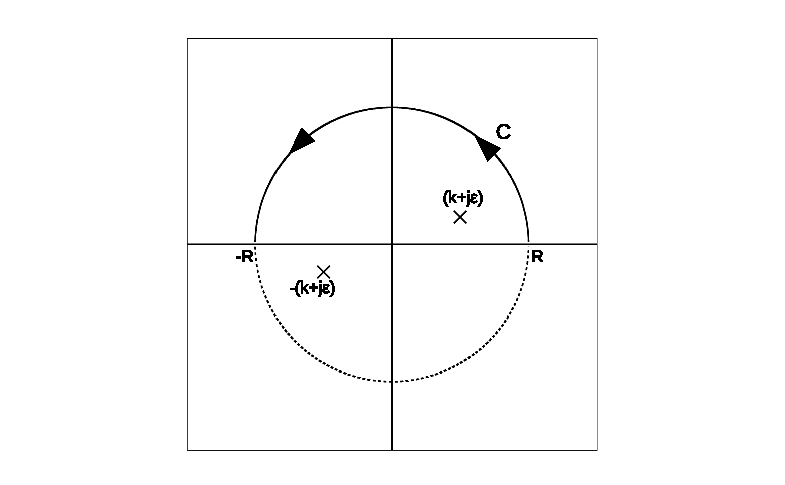
\includegraphics[width = 10cm]{./EPS/figure1new.eps}
    \label{fig1}
  \end{figure}
  \begin{eqnarray}
    F_+ = \int_{C} dk'\frac{e^{ik'(x-x')}}{(k'+k+i\epsilon)(k'-k-i\epsilon)} = \int_{-R}^Rdk' f_+(k') + \int_{C_1}dk'f_+(k')\label{c-int}
  \end{eqnarray}
  ただし
  \begin{eqnarray}
    f_+(k') = \frac{e^{ik'(x-x')}}{(k'+k+i\epsilon)(k'-k-i\epsilon)}
  \end{eqnarray}
  ここで留数定理
  \begin{eqnarray}
    \int_Cdz f(z) = 2\pi i\sum_j R(a_j)
  \end{eqnarray}
  を用いる. 極を$a_j$, Laurent展開における$(z-a)^{-n}$の係数を$R(a)$としている.今回の積分には1位の極しか含まれていないのでLaurent展開は
  \begin{eqnarray}
    R(a) = \lim_{z \rightarrow a}(z-a)f(z)
  \end{eqnarray}
  で与えられる. 以上より, (\ref{c-int})は
  \begin{eqnarray}
    F_+ &=& 2\pi i\lim_{k' \rightarrow k + j\epsilon }\left[(k'-k-j\epsilon)\frac{e^{ik'(x-x')}}{(k'+k+i\epsilon)(k'-k-i\epsilon)}\right]\\
    &=& \pi i\frac{e^{i(x-x')(k+j\epsilon)}}{k+j\epsilon}
  \end{eqnarray}
  と計算できる. さらに
  \begin{eqnarray}
    \lim_{R\rightarrow\infty}\int_{C_1}dk'f_+(k') =0
  \end{eqnarray}
  であることはすぐにわかる. 以上から
  \begin{eqnarray}
    G^\epsilon_+(x, x') &=& -\frac{1}{2\pi}\pi i\frac{e^{i(x-x')(k+j\epsilon)}}{k+j\epsilon}\\
    \therefore G_+(x, x') &=& \lim_{\epsilon\rightarrow 0}G_+^\epsilon(x, x') = -\frac{i}{2k}e^{ik(x-x')}
  \end{eqnarray}
  のように, Green関数を具体的に計算できた.\\
\item[ii)] $x<x'$の場合    
  \begin{figure}[htbp]
    \centering
    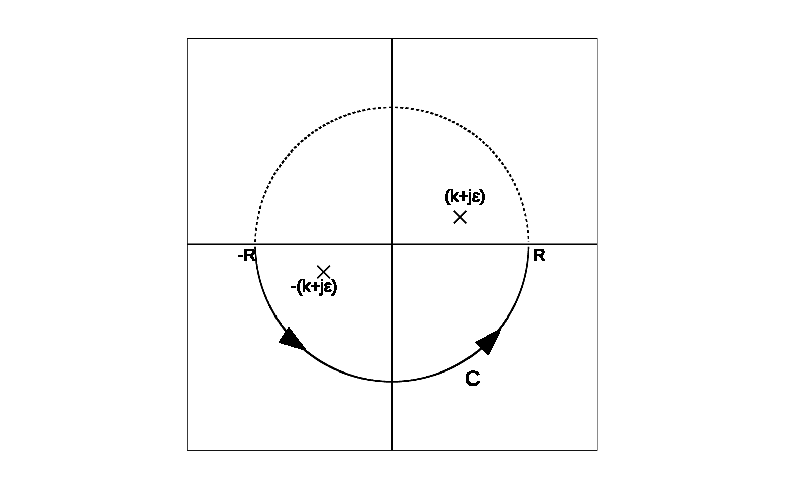
\includegraphics[width = 10cm]{./EPS/figure2new.eps}
    \label{fig2}
  \end{figure}
  先程と同様の計算より,
  \begin{eqnarray}
    G_-(x, x') = -\frac{i}{2k}e^{-ik(x-x')}
  \end{eqnarray}
  となる. 
\end{itemize}
まとめると,
\begin{eqnarray}
  G_\pm(x, x') = -\frac{i}{2k}e^{\pm ik(x-x')}
\end{eqnarray}
グリーン関数が求まったので, これを用いて波動関数を求める. 波動関数の摂動展開は
\begin{eqnarray}
  \psi(x) = \psi_0(x) + \int dx'G_+(x, x')H_p(x')\psi(x')
\end{eqnarray}
と表される.$\psi_0(x)$は非摂動解なので平面波であり, $H_p$はポテンシャルである. つまり, 領域ごとに$H_p$を変えてこの積分を計算すれば良い.
\section{場の理論におけるGreen関数}
場の理論と書きましたが, 以下では第二量子化された量子力学\footnote{「第二量子化された量子力学」と「場の量子論」は明確に区別されるべきです. 量子力学はあくまでSchr\"odinger方程式によって真空(基底状態)が決まるが, 場の量子論では真空は理論を閉じるように選ぶものである. 第二量子化における真空は消滅演算子$a$が消去する状態で確定しますが, 場の量子論においては真空期待値$\bra{0}\psi\ket{0}$がゼロでない値を持つことが許されます. こういう構造がないと, 粒子が存在する状態を真空とするBECのような物理を記述できなくなります.}におけるGreen関数についてまとめます.
\subsection{時間依存自由粒子Green関数}
場の演算子$\psi(\bm{x}, t)$はSchr\"odinger方程式
\begin{eqnarray}
  \left(i\hbar\partial_t -H\right)\psi(\bm{x}, t) = 0
\end{eqnarray}
で記述される. 今までの1粒子波動関数と同様に, 非摂動部のGreen演算子は
\begin{eqnarray}
  G_0(\bm{x}, t) = \left(i\hbar\partial_t -H_0\right)^{-1}
\end{eqnarray}
と表せ, グリーン関数は
\begin{eqnarray}
  \left(i\hbar\partial_t -H_0\right)G_0(\bm{x}, \bm{x}'; t, t') = \delta(t-t')\delta(\bm{x} - \bm{x}')
\end{eqnarray}
である. この微分方程式の解は2つ存在する:
\begin{eqnarray}
  G_0^R(k, \tau) &=& -i\theta(\tau)e^{-iE_k\tau}\hspace{1cm}\tau = t-t'\\
  G_0^A(k, \tau) &=& i\theta(\tau)e^{-iE_k\tau}\hspace{1cm}\tau = t'-t
\end{eqnarray}
$G^R$を遅延グリーン関数, $G^A$を先進グリーン関数と呼ぶ. 現象が時間に対して未来に進むのが遅延グリーン関数, 過去に進むのが先進グリーン関数になっている\footnote{数学的には時間が反転するような解を持っていてもおかしくないし, むしろ持っているべき. 時間発展がユニタリーなら解は時間反転対称性がある. }. 因果律を考慮しなくて良い場合であればどちらを用いてもよいが, 遅延グリーン関数の方が物理的な直感と合致している.
\subsection{相関関数と温度Green関数}
系が熱平衡状態にあるとき, $t = 0$の基底状態$\ket{\psi(0)}$を用いてGreen関数は, 可観測量$A, B$の時間相関関数で与えられる\footnote{Green関数が系に何かしらの揺動を与えた時の応答と解釈するなら自然な定義と言える.}:
\begin{eqnarray}
  G(t-t') \equiv \expval{\expval{A(t)B(t')}} = -i\bra{\psi(0)}{\rm T}[A(t)B(t')]\ket{0}
\end{eqnarray}
$A(t), B(t')$はHeisenberg描像, ${\rm T}[\ ]$は時間順序積. T積は因果律を守るために導入されている.

有限温度系における期待値は
\begin{eqnarray}
  \expval{A} = \frac{{\rm Tr}Ae^{-\beta H}}{{\rm Tr}e^{-\beta H}}
\end{eqnarray}
で与えられるので, 上のGreen関数は
\begin{eqnarray}
  G(t-t') &=& -i\frac{{\rm T}[{\rm Tr}A(t)B(t')e^{-\beta H}]}{{\rm Tr}e^{-\beta H}}\\
  &=& -i\frac{{\rm T}[{\rm Tr}e^{iHt/\hbar}Ae^{-iHt/\hbar}e^{iHt/\hbar}Be^{-iHt/\hbar}e^{-\beta H}]}{{\rm Tr}e^{-\beta H}}\\
  &=& -i\frac{{\rm T}[{\rm Tr}e^{iHt/\hbar}ABe^{-(it/\hbar + \beta)H}]}{{\rm Tr}e^{-\beta H}}
\end{eqnarray}
これを温度Green関数(松原Green関数)と呼ぶ.

